\documentclass[12pt]{article}

% Language setting
% Replace `english' with e.g. `spanish' to change the document language
\usepackage[english]{babel}

% Set page size and margins
% Replace `letterpaper' with`a4paper' for UK/EU standard size
\usepackage[letterpaper,top=2cm,bottom=2cm,left=3cm,right=3cm,marginparwidth=1.75cm]{geometry}


%AMS-TeX packages
\usepackage{amssymb,amsmath,amsthm} 
\usepackage{geometry, graphicx}
\usepackage{tabulary}
\usepackage{physics}
\usepackage{enumitem}


% setup the margins
\geometry{margin=1.0in, headheight=15pt}

\usepackage[colorlinks=true, allcolors=blue]{hyperref}
%% Common Declarations %%


\title{PHSX 425, Exam 02}
\author{William Jardee}

\begin{document}
\maketitle

\section*{8.2}
\emph{Consider the charging capacitor in Prob. 7.34}
\begin{figure}[h]
\centering
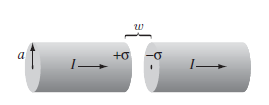
\includegraphics[scale=1]{homework08_question1.png}
\caption{Diagram from question 7.34}
\label{fig:1.1}
\end{figure}
\begin{enumerate}[label=\alph*)]
\item \emph{Find the electric and magnetic fields in the gap, as functions of distance $s$ from the axis and the time $t$. (Assume the charge is zero at $t=0$.)}\bigskip

\item \emph{Find the energy density $u_\text{em}$ and the Poynting vector $S$ in the gap. Note especially the direction of $S$. Check that Eq 8.12 is satisfied.}\bigskip

\item \emph{Determine the total energy in the gap, as a function of time. Calculate the total power flowing into the gap, by integrating the Poynting vector over the appropriate surface. Check that the power input is equal to the rate of increase of energy in the gap (Eq. 8.9 - in this case $W=0$, because there is no charge in the gap). [If you're worried about the fringing fields, do it for a volume of radius $b<a$ well inside the gap.]}\bigskip
\end{enumerate}

\section*{Question 2:}
\emph{The tip of a scanning tunneling microscope $(\theta < \alpha$, where $\alpha < \pi/2)$, held at a potential $V_0$, contacts a solid surface $(z=0)$. Assume that the STM tip and the surface it contacts are perfect conductors, but that the point of contact at the origin has resistance $R$. Find the Poynting vector $S$. Then calculate the Poynting flux, $\oint S\cdot \dd{a}$, through a shell of radius $r$ around the resistor.}\bigskip


\end{document}